\section{RESULTS}

\subsection{Experimental Data and Calculations}
The experimental results for various gas flow rates ($G\%$) and liquid irrigation rates ($L$) are presented below. The pressure drop per unit height ($\Delta P/Z$), friction factor ($f$), Reynolds number ($Re$), and the $\sigma$ factor were calculated for each data point.

% Table for L=0.0
\begin{table}[H]
    \centering
    \caption{Experimental results for $L=0.0$ gal/min}
    \begin{tabular}{ccccccc}
        \hline
        $G [\%]$ & $G [kg/s.m^2]$ & $\Delta P [mmH_2O]$ & $\Delta P/Z [N/m^3]$ & $\sigma$ & $f_{wet}$ & $Re$ \\
        \hline
        10 & 0.0847 & 1.0 & 23.36 & 1.00 & 4.02 & 46.86 \\
        20 & 0.1694 & 5.0 & 116.79 & 1.00 & 5.02 & 93.73 \\
        30 & 0.2541 & 10.0 & 233.57 & 1.00 & 4.47 & 140.59 \\
        40 & 0.3388 & 19.0 & 443.79 & 1.00 & 4.79 & 187.45 \\
        50 & 0.4235 & 29.0 & 677.36 & 1.00 & 4.75 & 234.32 \\
        60 & 0.5083 & 38.0 & 887.57 & 1.00 & 4.31 & 281.18 \\
        70 & 0.5930 & 52.0 & 1214.57 & 1.00 & 4.28 & 328.04 \\
        80 & 0.6776 & 70.0 & 1635.00 & 1.00 & 4.41 & 374.91 \\
        90 & 0.7623 & 90.0 & 2102.14 & 1.00 & 4.48 & 421.77 \\
        100 & 0.8471 & 108.0 & 2522.57 & 1.00 & 4.35 & 468.63 \\
        \hline
    \end{tabular}
\end{table}

% Table for L=0.2
\begin{table}[H]
    \centering
    \caption{Experimental results for $L=0.2$ gal/min}
    \begin{tabular}{ccccccc}
        \hline
        $G [\%]$ & $G [kg/s.m^2]$ & $\Delta P [mmH_2O]$ & $\Delta P/Z [N/m^3]$ & $\sigma$ & $f_{wet}$ & $Re$ \\
        \hline
        10 & 0.0847 & 1.0 & 23.36 & 1.00 & 4.02 & 46.86 \\
        20 & 0.1694 & 6.0 & 140.14 & 1.20 & 6.02 & 93.73 \\
        30 & 0.2541 & 12.0 & 280.29 & 1.20 & 5.37 & 140.59 \\
        40 & 0.3388 & 22.0 & 513.86 & 1.16 & 5.54 & 187.45 \\
        50 & 0.4235 & 32.0 & 747.43 & 1.10 & 5.24 & 234.32 \\
        60 & 0.5083 & 46.0 & 1074.43 & 1.21 & 5.21 & 281.18 \\
        70 & 0.5930 & 62.0 & 1448.14 & 1.19 & 5.10 & 328.04 \\
        80 & 0.6776 & 82.0 & 1915.14 & 1.17 & 5.17 & 374.91 \\
        90 & 0.7623 & 108.0 & 2522.57 & 1.20 & 5.37 & 421.77 \\
        100 & 0.8471 & 141.0 & 3292.50 & 1.31 & 5.68 & 468.63 \\
        \hline
    \end{tabular}
\end{table}

% Table for L=0.4
\begin{table}[H]
    \centering
    \caption{Experimental results for $L=0.4$ gal/min}
    \begin{tabular}{ccccccc}
        \hline
        $G [\%]$ & $G [kg/s.m^2]$ & $\Delta P [mmH_2O]$ & $\Delta P/Z [N/m^3]$ & $\sigma$ & $f_{wet}$ & $Re$ \\
        \hline
        10 & 0.0847 & 1.0 & 23.36 & 1.00 & 4.02 & 46.86 \\
        20 & 0.1694 & 8.0 & 186.86 & 1.60 & 8.03 & 93.73 \\
        30 & 0.2541 & 16.0 & 373.71 & 1.60 & 7.15 & 140.59 \\
        40 & 0.3388 & 26.0 & 607.29 & 1.37 & 6.55 & 187.45 \\
        50 & 0.4235 & 42.0 & 980.93 & 1.45 & 6.87 & 234.32 \\
        60 & 0.5083 & 62.0 & 1448.14 & 1.63 & 7.03 & 281.18 \\
        70 & 0.5930 & 109.0 & 2545.93 & 2.10 & 8.97 & 328.04 \\
        80 & 0.6776 & 172.0 & 4017.43 & 2.46 & 10.84 & 374.91 \\
        90 & 0.7623 & 267.0 & 6236.14 & 2.97 & 13.28 & 421.77 \\
        100 & 0.8471 & 315.0 & 7357.50 & 2.92 & 12.69 & 468.63 \\
        \hline
    \end{tabular}
\end{table}

% Table for L=0.6
\begin{table}[H]
    \centering
    \caption{Experimental results for $L=0.6$ gal/min}
    \begin{tabular}{ccccccc}
        \hline
        $G [\%]$ & $G [kg/s.m^2]$ & $\Delta P [mmH_2O]$ & $\Delta P/Z [N/m^3]$ & $\sigma$ & $f_{wet}$ & $Re$ \\
        \hline
        10 & 0.0847 & 0.0 & 0.00 & 0.00 & 0.00 & 46.86 \\
        20 & 0.1694 & 4.0 & 93.43 & 0.80 & 4.02 & 93.73 \\
        30 & 0.2541 & 17.0 & 397.07 & 1.70 & 7.60 & 140.59 \\
        40 & 0.3388 & 31.0 & 724.07 & 1.63 & 7.81 & 187.45 \\
        50 & 0.4235 & 49.0 & 1144.50 & 1.69 & 8.02 & 234.32 \\
        60 & 0.5083 & 95.0 & 2218.93 & 2.50 & 10.77 & 281.18 \\
        70 & 0.5930 & 174.0 & 4064.14 & 3.35 & 14.33 & 328.04 \\
        80 & 0.6776 & 295.0 & 6890.36 & 4.21 & 18.59 & 374.91 \\
        90 & 0.7623 & 377.0 & 8805.43 & 4.19 & 18.75 & 421.77 \\
        100 & 0.8471 & 434.0 & 10136.57 & 4.02 & 17.48 & 468.63 \\
        \hline
    \end{tabular}
\end{table}

% Table for L=0.8
\begin{table}[H]
    \centering
    \caption{Experimental results for $L=0.8$ gal/min}
    \begin{tabular}{ccccccc}
        \hline
        $G [\%]$ & $G [kg/s.m^2]$ & $\Delta P [mmH_2O]$ & $\Delta P/Z [N/m^3]$ & $\sigma$ & $f_{wet}$ & $Re$ \\
        \hline
        10 & 0.0847 & 2.0 & 46.71 & 2.00 & 8.03 & 46.86 \\
        20 & 0.1694 & 8.0 & 186.86 & 1.60 & 8.03 & 93.73 \\
        30 & 0.2541 & 20.0 & 467.14 & 2.00 & 8.94 & 140.59 \\
        40 & 0.3388 & 53.0 & 1237.93 & 2.79 & 13.36 & 187.45 \\
        50 & 0.4235 & 107.0 & 2499.21 & 3.69 & 17.52 & 234.32 \\
        60 & 0.5083 & 164.0 & 3830.36 & 4.32 & 18.59 & 281.18 \\
        70 & 0.5930 & 348.0 & 8128.29 & 6.69 & 28.66 & 328.04 \\
        80 & 0.6776 & 412.0 & 9622.93 & 5.89 & 25.96 & 374.91 \\
        \hline
    \end{tabular}
\end{table}

% Table for L=1.0
\begin{table}[H]
    \centering
    \caption{Experimental results for $L=1.0$ gal/min}
    \begin{tabular}{ccccccc}
        \hline
        $G [\%]$ & $G [kg/s.m^2]$ & $\Delta P [mmH_2O]$ & $\Delta P/Z [N/m^3]$ & $\sigma$ & $f_{wet}$ & $Re$ \\
        \hline
        10 & 0.0847 & 3.0 & 70.07 & 3.00 & 12.05 & 46.86 \\
        20 & 0.1694 & 9.0 & 210.21 & 1.80 & 9.03 & 93.73 \\
        30 & 0.2541 & 23.0 & 537.21 & 2.30 & 10.28 & 140.59 \\
        40 & 0.3388 & 49.0 & 1144.50 & 2.58 & 12.35 & 187.45 \\
        50 & 0.4235 & 95.0 & 2218.93 & 3.28 & 15.55 & 234.32 \\
        60 & 0.5083 & 180.0 & 4204.29 & 4.74 & 20.40 & 281.18 \\
        70 & 0.5930 & 303.0 & 7077.21 & 5.83 & 24.95 & 328.04 \\
        80 & 0.6776 & 393.0 & 9179.14 & 5.61 & 24.77 & 374.91 \\
        \hline
    \end{tabular}
\end{table}

% Table for L=1.2
\begin{table}[H]
    \centering
    \caption{Experimental results for $L=1.2$ gal/min}
    \begin{tabular}{ccccccc}
        \hline
        $G [\%]$ & $G [kg/s.m^2]$ & $\Delta P [mmH_2O]$ & $\Delta P/Z [N/m^3]$ & $\sigma$ & $f_{wet}$ & $Re$ \\
        \hline
        10 & 0.0847 & 3.0 & 70.07 & 3.00 & 12.05 & 46.86 \\
        20 & 0.1694 & 14.0 & 327.00 & 2.80 & 14.05 & 93.73 \\
        30 & 0.2541 & 35.0 & 817.50 & 3.50 & 15.64 & 140.59 \\
        40 & 0.3388 & 75.0 & 1751.79 & 3.95 & 18.90 & 187.45 \\
        50 & 0.4235 & 163.0 & 3807.00 & 5.62 & 26.68 & 234.32 \\
        60 & 0.5083 & 246.0 & 5745.86 & 6.47 & 27.88 & 281.18 \\
        70 & 0.5930 & 332.0 & 7754.79 & 6.38 & 27.34 & 328.04 \\
        80 & 0.6776 & 418.0 & 9763.07 & 5.97 & 26.34 & 374.91 \\
        \hline
    \end{tabular}
\end{table}

% Table for L=1.4
\begin{table}[H]
    \centering
    \caption{Experimental results for $L=1.4$ gal/min}
    \begin{tabular}{ccccccc}
        \hline
        $G [\%]$ & $G [kg/s.m^2]$ & $\Delta P [mmH_2O]$ & $\Delta P/Z [N/m^3]$ & $\sigma$ & $f_{wet}$ & $Re$ \\
        \hline
        10 & 0.0847 & 5.0 & 116.79 & 5.00 & 20.09 & 46.86 \\
        20 & 0.1694 & 20.0 & 467.14 & 4.00 & 20.07 & 93.73 \\
        30 & 0.2541 & 62.0 & 1448.14 & 6.20 & 27.71 & 140.59 \\
        40 & 0.3388 & 118.0 & 2756.14 & 6.21 & 29.74 & 187.45 \\
        50 & 0.4235 & 328.0 & 7660.93 & 11.31 & 53.70 & 234.32 \\
        \hline
    \end{tabular}
\end{table}

% Table for L=1.6
\begin{table}[H]
    \centering
    \caption{Experimental results for $L=1.6$ gal/min}
    \begin{tabular}{ccccccc}
        \hline
        $G [\%]$ & $G [kg/s.m^2]$ & $\Delta P [mmH_2O]$ & $\Delta P/Z [N/m^3]$ & $\sigma$ & $f_{wet}$ & $Re$ \\
        \hline
        10 & 0.0847 & 8.0 & 186.86 & 8.00 & 32.14 & 46.86 \\
        20 & 0.1694 & 25.0 & 583.93 & 5.00 & 25.09 & 93.73 \\
        30 & 0.2541 & 78.0 & 1821.86 & 7.80 & 34.86 & 140.59 \\
        40 & 0.3388 & 142.0 & 3316.43 & 7.47 & 35.79 & 187.45 \\
        50 & 0.4235 & 258.0 & 6026.57 & 8.90 & 42.24 & 234.32 \\
        \hline
    \end{tabular}
\end{table}

\begin{figure}[H]
    \centering
    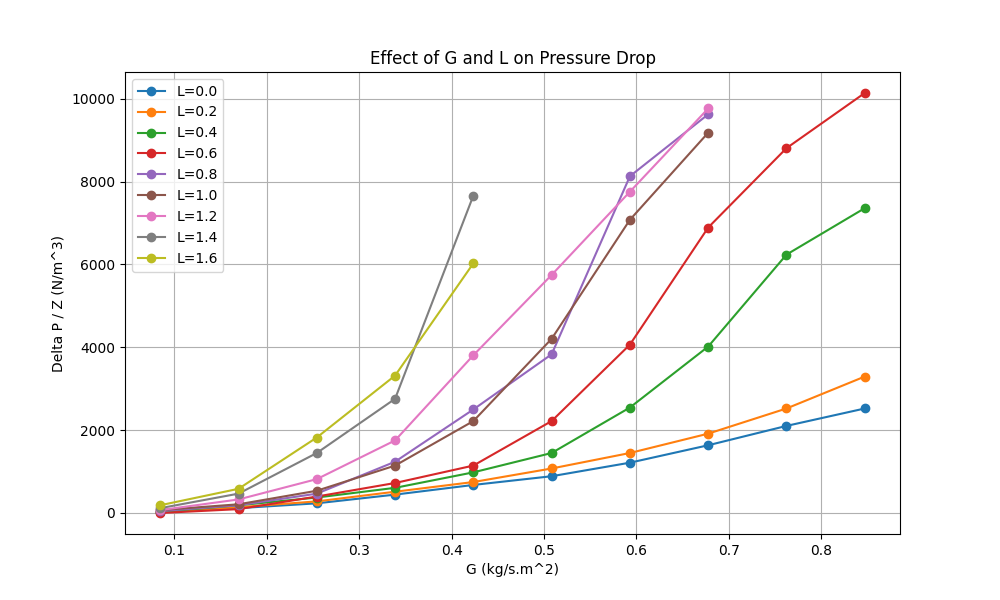
\includegraphics[width=0.8\textwidth]{Images/dp_chart.png}
    \caption{Effect of gas flow rate $G$ and liquid irrigation rate $L$ on the pressure drop $\Delta P/Z$.}
\end{figure}

\begin{figure}[H]
    \centering
    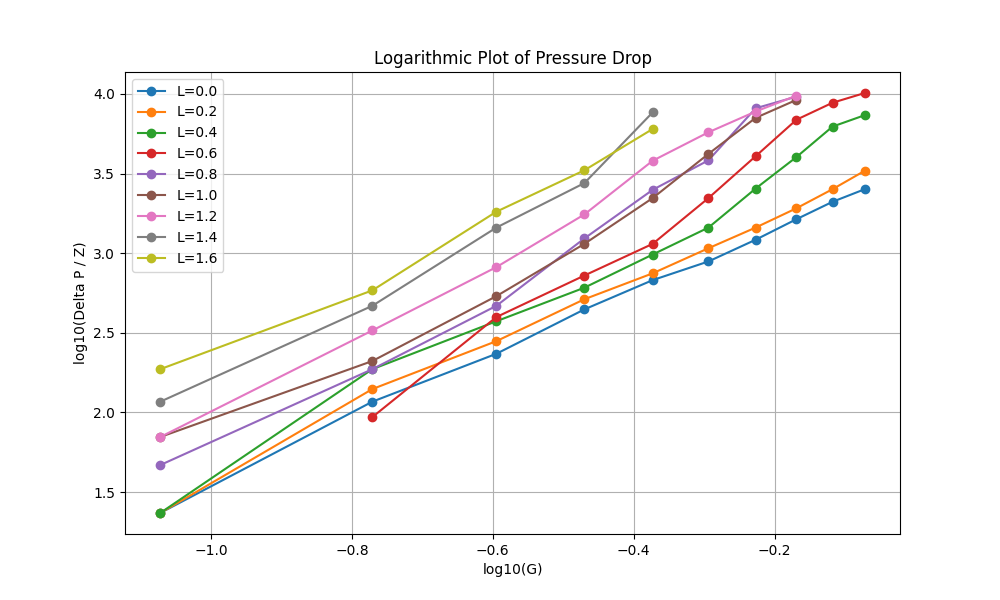
\includegraphics[width=0.8\textwidth]{Images/log_dp_chart.png}
    \caption{Logarithmic plot of pressure drop vs. gas flow rate.}
\end{figure}

\subsection{Flooding Point Analysis}
The flooding point was identified for each liquid irrigation rate. The dimensionless numbers $\pi_1$ and $\pi_2$ were calculated to determine the flooding limit of the packed column.

\begin{table}[H]
    \centering
    \caption{Flooding point data for different liquid flow rates}
    \begin{tabular}{cccccccc}
        \hline
        $L [gal/min]$ & $G^* [\%]$ & $G^* [kg/s.m^2]$ & $v [m/s]$ & $\pi_1$ & $\pi_2$ & $\log \pi_1$ & $\log \pi_2$ \\
        \hline
        0.2 & 100 & 0.8471 & 0.7493 & 0.2583 & 0.0952 & -0.5879 & -1.0215 \\
        0.4 & 100 & 0.8471 & 0.7493 & 0.2583 & 0.1903 & -0.5879 & -0.7205 \\
        0.6 & 100 & 0.8471 & 0.7493 & 0.2583 & 0.2855 & -0.5879 & -0.5444 \\
        0.8 & 80 & 0.6776 & 0.5994 & 0.1674 & 0.4759 & -0.7762 & -0.3225 \\
        1.0 & 80 & 0.6776 & 0.5994 & 0.1674 & 0.5948 & -0.7762 & -0.2256 \\
        1.2 & 80 & 0.6776 & 0.5994 & 0.1674 & 0.7138 & -0.7762 & -0.1464 \\
        1.4 & 50 & 0.4235 & 0.3746 & 0.0694 & 1.3324 & -1.1589 & 0.1246 \\
        1.6 & 50 & 0.4235 & 0.3746 & 0.0694 & 1.5227 & -1.1589 & 0.1826 \\
        \hline
    \end{tabular}
\end{table}

\begin{figure}[H]
    \centering
    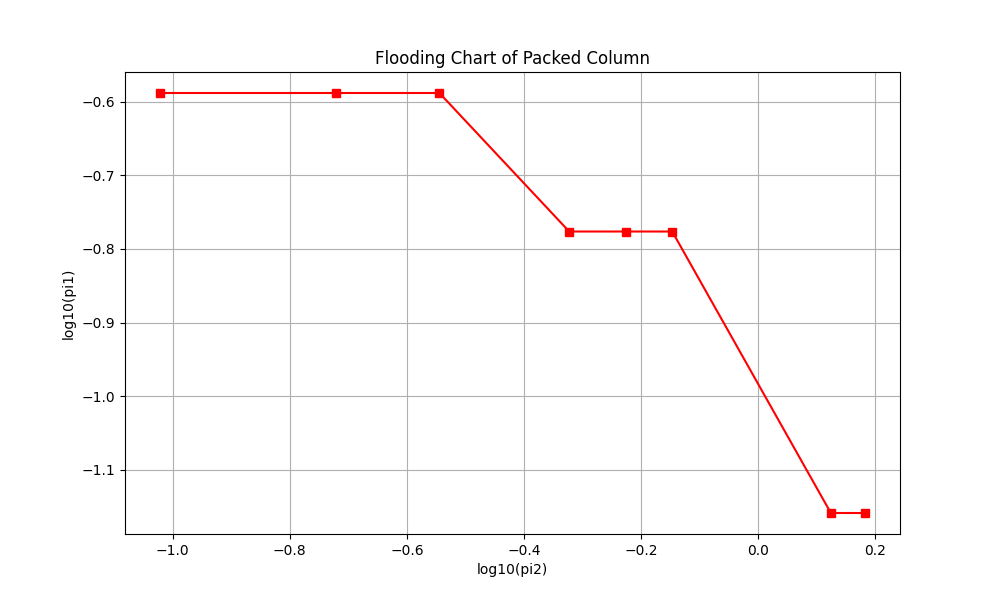
\includegraphics[width=0.8\textwidth]{Images/flooding_chart.png}
    \caption{Flooding chart of the packed column ($\log \pi_1$ vs. $\log \pi_2$).}
\end{figure}

\subsection{Empirical Results and Equations}
The relationship between the hydrodynamic parameters was analyzed using regression analysis. Table \ref{tab:empirical} summarizes the empirical equations derived from the experimental data.

\begin{table}[H]
    \centering
    \caption{The empirical results and equations}
    \label{tab:empirical}
    \begin{tabular}{ll}
        \hline
        \textbf{Relation} & \textbf{Empirical Equation} \\
        \hline
        $\Delta P_{ck}/Z$ vs $G$ at $L = 0$ & $y = 3070.4x^2 + 359.51x - 8.9536$ \\
        $\Delta P_{c\ddot{o}}/Z$ vs $G$ at $L = 0.2$ & $y = 3723.9x^2 - 28.828x + 56.836$ \\
        $\Delta P_{c\ddot{o}}/Z$ vs $G$ at $L = 0.4$ & $y = 4784.4x^2 - 30.917x + 28.029$ \\
        $\Delta P_{c\ddot{o}}/Z$ vs $G$ at $L = 0.6$ & $y = 9146x^2 - 1549.4x + 184.35$ \\
        $\Delta P_{c\ddot{o}}/Z$ vs $G$ at $L = 0.8$ & $y = 17323x^2 - 4402.1x + 397.07$ \\
        $\Delta P_{c\ddot{o}}/Z$ vs $G$ at $L = 1$ & $y = 11702x^2 - 1448.7x + 109.08$ \\
        $\Delta P_{c\ddot{o}}/Z$ vs $G$ at $L = 1.2$ & $y = 35809x^2 - 6342.2x + 385.39$ \\
        $\Delta P_{c\ddot{o}}/Z$ vs $G$ at $L = 1.4$ & $y = 35809x^2 - 6342.2x + 385.39$ \\
        $\Delta P_{c\ddot{o}}/Z$ vs $G$ at $L = 1.6$ & $y = 23601x^2 - 3240x + 198.54$ \\
        \hline
        $\log f_{ck}$ vs $Re_{ck}$ at $L = 0$ & $y = -0.0006x + 0.8656$ \\
        $\log f_{c\ddot{o}}$ vs $Re_{ck}$ at $L = 0.2$ & $y = -0.0007x + 0.9235$ \\
        $\log f_{c\ddot{o}}$ vs $Re_{ck}$ at $L = 0.4$ & $y = -0.0006x + 0.9861$ \\
        $\log f_{c\ddot{o}}$ vs $Re_{ck}$ at $L = 0.6$ & $y = -0.0005x + 1.046$ \\
        $\log f_{c\ddot{o}}$ vs $Re_{ck}$ at $L = 0.8$ & $y = -0.0002x + 1.0543$ \\
        $\log f_{c\ddot{o}}$ vs $Re_{ck}$ at $L = 1$ & $y = 0.0003x + 1.1032$ \\
        $\log f_{c\ddot{o}}$ vs $Re_{ck}$ at $L = 1.2$ & $y = 0.0011x + 1.0434$ \\
        $\log f_{c\ddot{o}}$ vs $Re_{ck}$ at $L = 1.4$ & $y = 0.0015x + 1.0995$ \\
        $\log f_{c\ddot{o}}$ vs $Re_{ck}$ at $L = 1.6$ & $y = 0.002x + 1.1082$ \\
        \hline
        $\log \sigma$ vs $L$ at $G = 10\%$ & $y = 0.13x - 0.001$ \\
        $\log \sigma$ vs $L$ at $G = 20\%$ & $y = 0.38x + 0.02$ \\
        $\log \sigma$ vs $L$ at $G = 30\%$ & $y = 0.42x - 0.02$ \\
        \hline
    \end{tabular}
\end{table}
